\documentclass[10pt,a4paper]{article}
\usepackage[utf8]{inputenc}
\usepackage{amsmath}
\usepackage{gensymb}
\usepackage{amsfonts}
\usepackage{siunitx}
\usepackage[european]{circuitikz}
\usepackage{geometry}
\newgeometry{tmargin=2cm, bmargin=2cm, lmargin=2cm, rmargin=2cm}
\usepackage{amssymb}
\usepackage{multirow}
\usepackage{polski}
\usepackage{graphicx}
\author{\textbf{T. Fąs}}
\title{\textbf{WZMACNIACZ OPERACYJNY}}
\begin{document}
\maketitle

\begin{center}
\textbf{\subsection*{STRESZCZENIE}}
\end{center}
W doświadczeniu zbadano właściwości wzmacniacza operacyjnego oraz skonstruowano układy oparte o ten wzmacniacz. Wszystkie konstrukcje zachowywały się zgodnie z oczekiwaniami.


\begin{center}
\textbf{\subsection*{WSTĘP}}
\end{center}
Wzmacniacz operacyjny jest układem realizującym operację wzmocnienia różnicy sygnałów wejściowych. Symbol wzmacniacza przedstawiony jest na Rysunku 1.

\begin{figure}[h!]
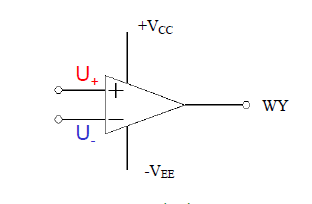
\includegraphics[width=6cm]{rap23rys1} 
\centering
\caption{Wzmacniacz operacyjny.}
\end{figure}

Jeżeli na wejście "+" znajduje się napięcie $U_{+}$, a na wejściu "-" napięcie $U_{-}$, to na wyjściu wzmacniacza otrzymamy sygnał $A(U_{+}-U_{-})$, gdzie $A$ jest pewną stałą wzmocnienia. Układ ten wymaga dodatkowo zasilania z dwóch źródeł, tu oznaczonych jako $V_{CC}$ i $V_{EE}$.


Korzystając z tego elementu można stworzyć: wzmacniacz odwracający fazę (sygnał na wyjściu ma przeciwną fazę), wzmacniacz nieodwracający fazy, układ różniczkujący (sygnał na wyjściu jest pochodną sygnału wejściowego) i układ całkujący. Schematy tych układów przedstawiono na Rysunku 2. 

\begin{figure}[h!]
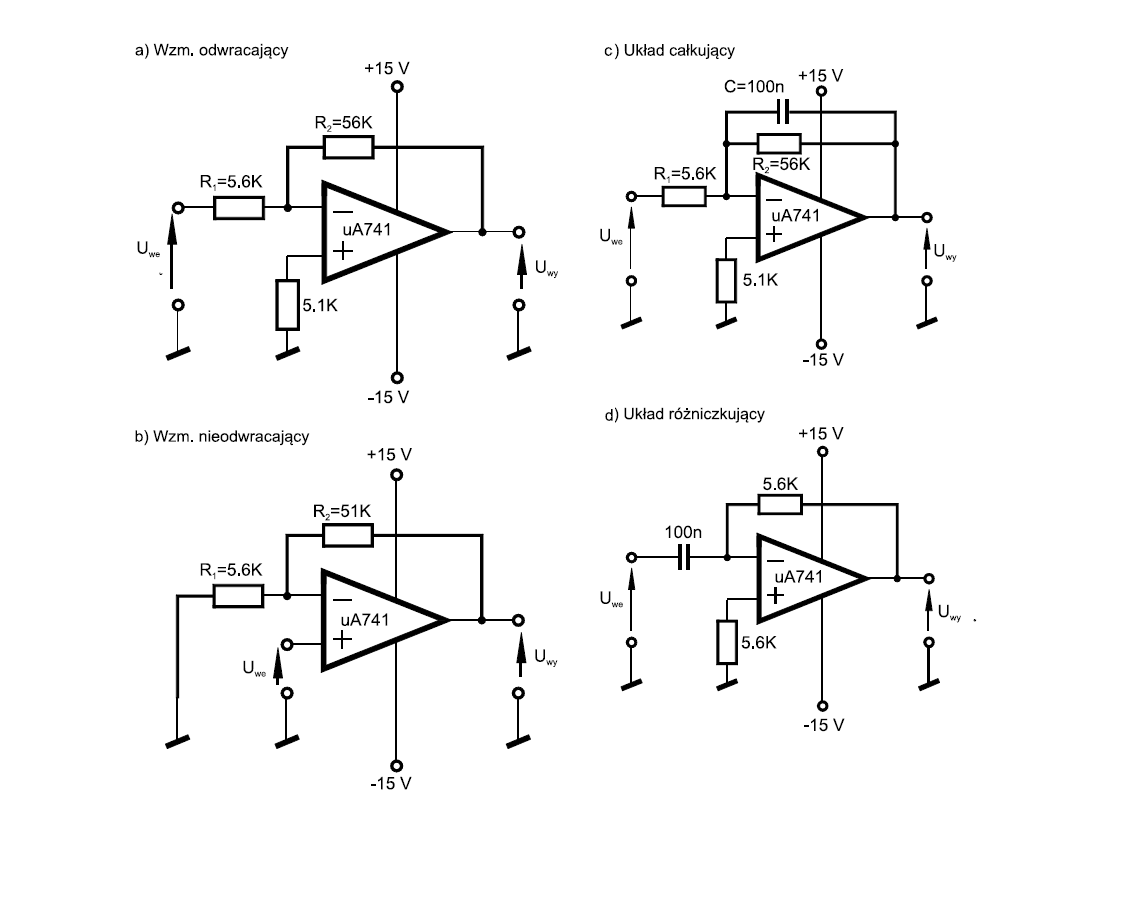
\includegraphics[width=12cm]{rap23rys2} 
\centering
\caption{Schematy układów \cite{r1}.}
\end{figure}

W przypadku wzmacniaczy, zależność napięcia wejściowego od wyjściowego jest zależnością liniową, a zależność napięcia wyjściowego $U_{wy}$ od częstości $\omega$ napięcia  wejściowego $U_{we}$ jest zależnością filtra dolnoprzepustowego, tj:

\begin{equation}
\left| \dfrac{U_{wy}}{U_{we}}\right|=\dfrac{k\omega_{g}}{\sqrt{\omega^2+\omega_{g}^2}},
\end{equation}

gdzie $k$ to stała wzmocnienia, a $\omega_{g}$ to częstość krytyczna, dla której stosunek napięć wynosi $1/\sqrt{2}$. 

\begin{center}
\textbf{\subsection*{UKŁAD DOŚWIADCZALNY}}
\end{center}


\begin{center}
\textbf{\subsection*{WYNIKI POMIARÓW}}
\end{center}

 

\begin{center}
\textbf{\subsection*{ANALIZA DANYCH}}
\end{center}



\begin{center}
\textbf{\subsection*{DYSKUSJA WYNIKÓW I WNIOSKI}}
\end{center} 





\begin{center}
\begin{thebibliography}{9}

\bibitem{r1}
 Praca zbiorowa,
 \emph{Instrukcja do ćwiczenia "Wzmacniacz operacyjny"},
 FUW, Warszawa, 2016.
 
 
 
 \end{thebibliography}

\end{center}


\end{document}